\section{Results}


\subsection{Effect of spatial structure in PD and HD games}
In our first simulation experiment, we compared the effect of spatial structure on the persistence of cooperators in the PD and HD games.





The regression shows a significant correlation between estimates and the attitude statement (figure \ref{fig: Regression}): The higher the estimated number of refugees, the more likely people oppose hosting more refugees.



\begin{figure}
	\centering 
	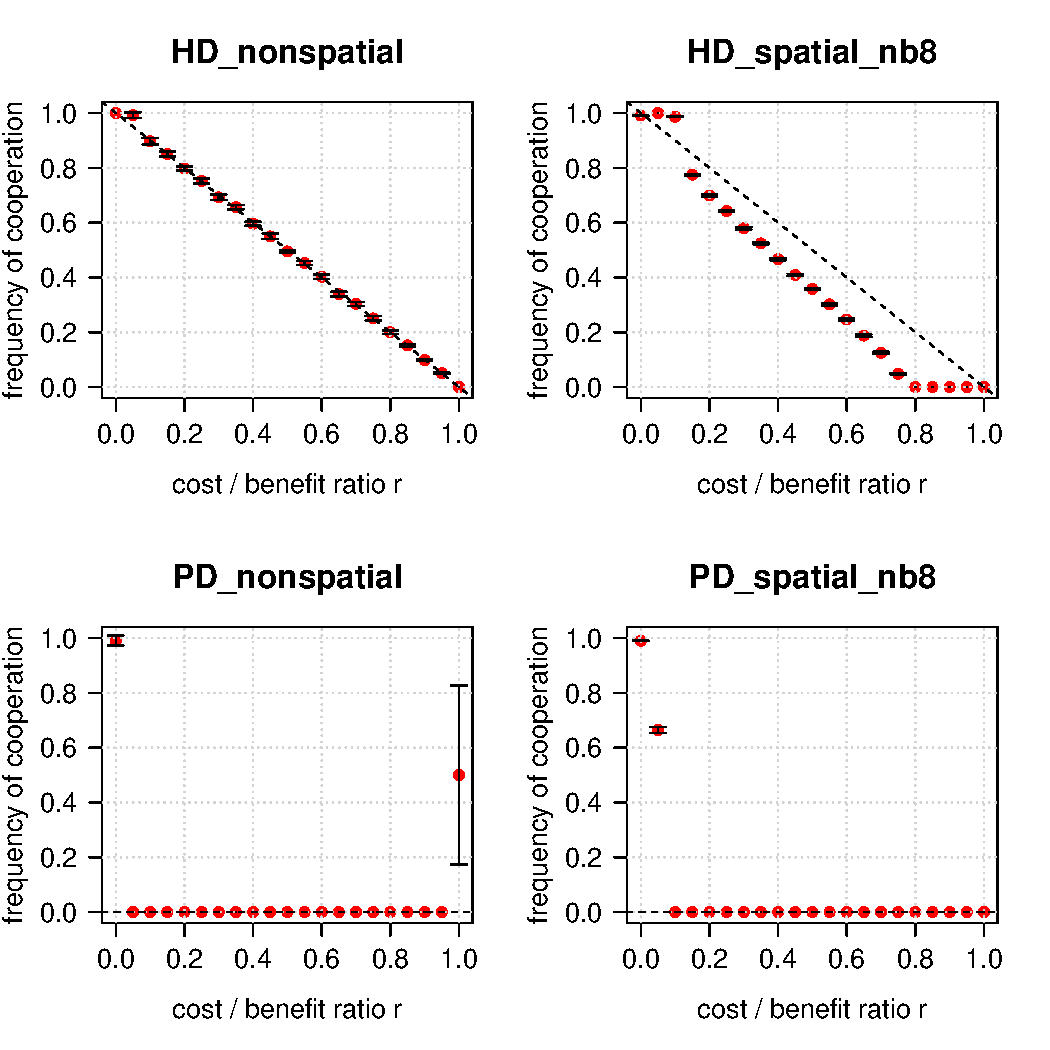
\includegraphics[width=9.5cm]{task1_4plot}
	\caption{Comparison of HD and PD game simulations, both with and without spatial structure.  \textbf{[ t = 5000, i = 10 ]} }\label{fig: task1_4plot}
\end{figure}


We produced a residual pattern plot and a Q-Q-Plot of the model to examine model quality. The residuals are nicely distributed in both Residual vs. fitted Plot and Q-Q-Plot (see figure \ref{fig: Q-Q-Plot}). Therefore we consider our model appropriate.
A summarizing box plot of our model including the regression line is given in figure \ref{fig: ModelPlot}.

In the second regression we correlated the logarithmized absolute difference between estimates and actual refugee number to the attitude records. Our data do not show a significant correlation between attitude and the difference to actual refugee numbers as a proxy for knowledge.



\begin{figure}[H]
	\centering 
	\includegraphics[width=7cm]{Q-Q-Plot}
	\caption{residual distribution and Q-Q-Plot of the fitted model}\label{fig: Q-Q-Plot}
\end{figure}


\begin{figure}[H]
	\centering 
	\includegraphics[width=7cm]{ModelPlot}
	\caption{Attitude towards refugees in dependence of estimated numbers. Blue = regression line}\label{fig: ModelPlot}
\end{figure}


\subsection{Effect of neighbourhood size}

In order to check for possible confounding factors, we conducted an analysis of variance for gender, age and place of interview.

\textbf{Gender:} There was no influence of gender on attitude. Surprisingly, statements by male and female are completely equally distributed, even though we were 5 researchers interviewing 124 people. 

\textbf{Age:} According to preliminary data analysis, people favoring more refugees were younger than people who favored keeping the same number or less refugees. However, the ANOVA we conducted to test for an influence of age was not significant (p-value = 0.7898). We therefore do not consider age a relevant confounding factor.

\textbf{Place:} Unlike with the other variables, the place where interviews were conducted had a significant influence on the attitudes expressed. The ANOVA we returned a p-value of 0.0386.
In Vauban and on campus, people were more positive towards refugees than in the hiking area or at the technical faculty (see figure \ref{fig: Place}).

\begin{figure}
	\centering 
	\includegraphics[width=7cm]{Place}
	\caption{Attitudes towards refugees at different places}\label{fig: Place}
\end{figure}


\subsection{Effect of mixed strategies}

